%*****************************************
\chapter{Unobtrusive Research}\label{ch12:unobtrusive}
%*****************************************

\section{Introduction}

\begin{wrapfigure}{r}{0.4\textwidth}
	\centering
	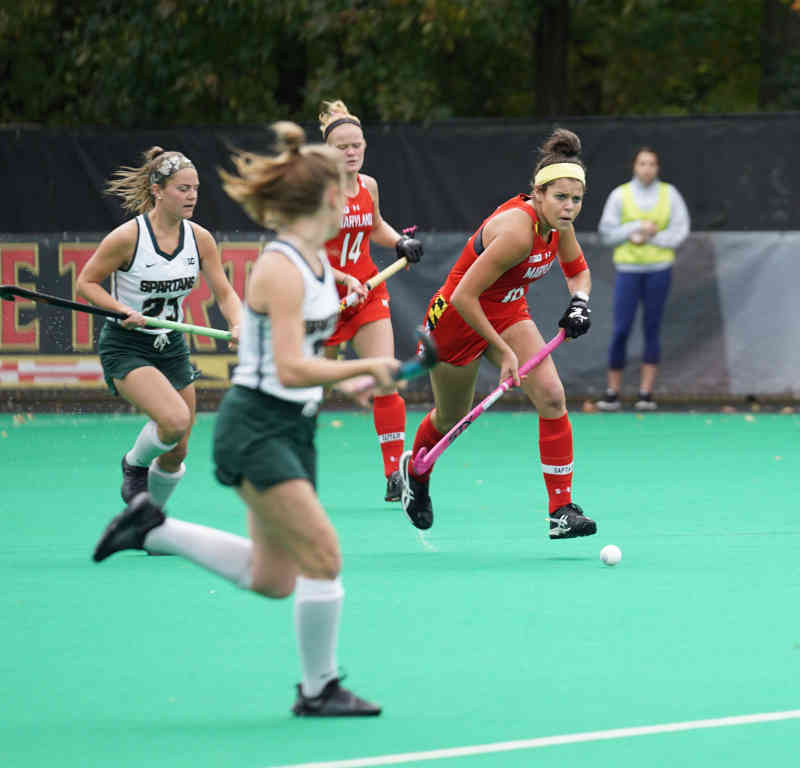
\includegraphics[width=0.4\textwidth]{gfx/12-women_hockey} 
\end{wrapfigure}

Are female and male athletes at the professional and college levels treated equally? It would be reasonable to think after 40 years since the passing of Title IX (the civil rights law that prohibits sex discrimination in education including athletics) and with the growing visibility of women athletes in sports such as golf, basketball, hockey, and tennis, that the answer would be an easy yes. But Professor Michael Messner's \cite{messner2002taking} unobtrusive research shows otherwise, as does Professors Jo Ann M. Buysse and Melissa Sheridan Embser-Herbert's \cite{buysse2004constructions} content analysis of college athletics media guide photographs. In fact, Buysse and Embser-Herbert's unobtrusive research shows that traditional definitions of femininity are fiercely maintained through colleges' visual representations of women athletes as passive and overtly feminine (as opposed to strong and athletic). Unobtrusive research made it possible to clear up misconceptions about changes for women athletes over the past 40 years.\blfootnote{Photo by Jeffrey F Lin on Unsplash}

\begin{center}
	\begin{objbox}{Objectives}
		\begin{itemize}
			\setlength{\itemsep}{0pt}
			\setlength{\parskip}{0pt}
			\setlength{\parsep}{0pt}
			
			\item Define ``Unobtrusive Research.''
			\item Describe the strengths and weaknesses of unobtrusive research.
			\item Describe methods used for unobtrusive data collection and analysis.
			\item Describe how data collected by others can be used.
			\item Discuss reliability in unobtrusive research.
		\end{itemize}
	\end{objbox}
\end{center}

\section{What Is Unobtrusive Research?}

This chapter explores unobtrusive methods of collecting data, which are methods that do not interfere with the subjects under study. Both qualitative and quantitative researchers use unobtrusive research methods. Unobtrusive methods share the unique quality that they do not require researchers to interact with the people they are studying. It may seem strange that business, a discipline dedicated to understanding human purchasing behavior, would employ a methodology that requires no interaction with human beings. But humans create plenty of evidence of their behaviors---they write letters to the editor of their local paper, they create various sources of entertainment for themselves such as movies and televisions shows, they consume goods, they walk on sidewalks, they lie on the grass in public parks. All these activities leave something behind---worn paths, trash, recorded shows, and printed papers. These are all potential sources of data for the unobtrusive researcher.

Unobtrusive research methods include content analysis, indirect measures, and using data collected by others. All of these methods are similar in that they do not require direct interaction between researchers and their human subjects but each has its unique qualities. This chapter also considers how data gathered unobtrusively can be analyzed and how reliability in that data can be improved.

\subsection{Strengths of Unobtrusive Research}

Researchers who seek evidence of what people actually do, as opposed to what they say they do (as in survey and interview research), might wish to consider using unobtrusive methods. Field researchers may also claim this advantage over interview and survey research, but field researchers cannot be certain about what effect their presence in the field may have on the people and the interactions that they observe. While unobtrusive research projects, like all research projects, face the risk of introducing researcher bias into the work, researchers employing unobtrusive methods do not need to be concerned about the effect of the research on their subjects. This effect, known as the \Gls{hawthorne} effect, is not a concern for unobtrusive researchers because they do not interact directly with their research participants. In fact, this is one of the major strengths of unobtrusive research.

Another benefit of unobtrusive research is that it can be relatively low-cost compared to some of the other research methods. Because ``participants'' are generally inanimate objects as opposed to human beings, researchers may be able to access data without having to worry about paying participants for their time (though certainly travel to or access to some documents and archives can be costly).

Unobtrusive research is also relatively forgiving. It is far easier to correct mistakes made in data collection when conducting unobtrusive research than when using any other method. Imagine the challenge, for example, if researchers realized at the end of conducting $ 50 $ in-depth interviews that they had accidentally omitted two critical questions from the interview guide. What options would they have? Re-interview all $ 50 $ participants? Try to figure out what respondents might have said based on their other responses? Re-frame the research question? Scratch the project entirely? Obviously none of these options are ideal. The same problems arise if a mistake is made in survey research. For field researchers, the consequences of ``messing up'' during data collection can be even more disastrous. Imagine discovering after tagging along on a political candidate's campaign that a ``do-over'' is needed. In this case, that simply is not an option. The campaign is over, and the researcher would need to find a new source of data. Fortunately for unobtrusive researchers, going back to the source of the data to gather more information or correct some problem in the original data collection is a relatively straightforward prospect.

Finally, unobtrusive research is well suited to studies that focus on processes that occur over time. While longitudinal surveys and long-term field observations are also suitable ways of gathering such information, they cannot examine processes that occurred decades before data collection began, nor are they the most cost-effective ways to examine long-ranging processes. Unobtrusive methods, on the other hand, enable researchers to investigate events and processes that have long since passed. They also do not rely on retrospective accounts, which may be subject to errors in memory, as some longitudinal surveys do.

\subsection{Weaknesses of Unobtrusive Research}

While there are many benefits to unobtrusive research, this method also comes with a unique set of drawbacks. Because unobtrusive researchers analyze data that may have been created or gathered for purposes entirely different from the researcher's goal, problems of validity sometimes arise in such projects. It may also be the case that data sources measuring whatever a researcher wishes to examine simply do not exist. This means that unobtrusive researchers may be forced to tweak their original research interests or questions to better suit the data that are available to them. Finally, it can be difficult in unobtrusive research projects to account for context. In a field research project, for example, the researcher is able to see what events lead up to some occurrence and observe how people respond to that occurrence. What this means for unobtrusive research is that while it can be difficult to ascertain why something occurred, we can gain a good understanding of what has occurred.

\section{Unobtrusive Data Collection}

This section focuses on unobtrusive data collection and what to do with those data once they have been collected. There are two main ways of gathering data unobtrusively: conducting a content analysis of existing texts and analyzing physical traces of human behavior, both explored here.

\subsection{Content Analysis}

One way of conducting unobtrusive research is to analyze texts, which come in all kinds of formats. At its core, content analysis addresses the questions of ``Who says what, to whom, why, how, and with what effect?''\cite{babbie2010practice}. Content analysis is a type of unobtrusive research that involves the study of human communications. Another way to think of content analysis is as a way of studying texts and their meaning. This is a more liberal definition of ``text'' than may be found in a dictionary. The text that content analysts investigate includes such things as actual written copy (\eg, newspapers or letters) and content that might be seen or heard (\eg, speeches or other performances). Content analysts might also investigate more visual representations of human communication such as television shows, photographs, advertisements, or movies.

As an example of content analysis, Braunsberger and Buckler \cite{braunsberger2011motivates} investigated why people participate in consumer boycotts. They analyzed comments submitted to an online boycott petition concerning Canadian Seafood. As a result of analyzing a sample of $ 1200 $ of the $ 17,496 $ boycott pledges, the researchers concluded that $ 70.1\% $ of the pledges wished the target to discontinue its egregious behavior and $ 29.67\% $ wanted to send a message to the target that the boycott would impact the company's bottom line. (Note, these two groups overlapped.) 

As a second example, Cheyne, Dorfman, and Bukofzer \cite{cheyne2013marketing} analyzed the websites of $ 16 $ different cereals marketed to children, such as \textit{Apple Jacks}, \textit{Cocoa Puffs}, and \textit{Lucky Charms}, and found that the sites used various progressive levels of presence to encourage children to engage with their products. The more successful sites, as measured by traffic data, featured activities with deeper ``levels of immersion,'' like advergames.

Both of these examples used unobtrusive techniques to measure phenomena. 

Content analysis is the systematic analysis of the content of a text (\eg, who says what, to whom, why, and to what extent and with what effect) in a quantitative or qualitative manner. Content analysis is typically conducted as follows. 

\begin{enumerate}
	\item When there are many texts to analyze (\eg, newspaper stories, financial reports, blog postings, online reviews, etc.), the researcher begins by sampling a selected set of texts from the population of texts for analysis. This process is not random, but instead, texts that have more pertinent content should be chosen selectively. 

	\item The researcher identifies and applies rules to divide each text into segments or ``chunks'' that can be treated as separate units of analysis. This process is called unitizing. For example, assumptions, effects, enablers, and barriers in texts may constitute such units.

	\item The researcher constructs and applies one or more concepts to each unitized text segment in a process called coding. For coding purposes, a coding scheme is used that is based on themes discovered as the text is classified.

	\item The coded data are analyzed, often both quantitatively and qualitatively, to determine which themes occur most frequently, in what contexts, and how they are related to each other.
\end{enumerate}

A simple type of content analysis is sentiment analysis which is a technique used to capture people's opinion or attitude toward an object, person, or phenomenon. Reading online messages about a political candidate posted to an online forum and classifying each message as positive, negative, or neutral is an example of such an analysis. In this case, each message represents one unit of analysis. This analysis will help identify whether the sample as a whole is positively or negatively disposed or neutral towards that candidate. Examining the content of online reviews in a similar manner is another example. Though this analysis can be done manually, for very large data sets (millions of text records), natural language processing and analytics programs are available to automate the coding process and maintain a record of how sentiments fluctuate with time.

A frequent criticism of content analysis is that it lacks a set of systematic procedures that would allow the analysis to be replicated by other researchers. Schilling\cite{schilling2006pragmatics} addressed this criticism by organizing different content analytic procedures into a spiral model. This model consists of five levels or phases in interpreting text: 

\begin{enumerate}
	\item convert recorded tapes into raw text data or transcripts for content analysis
	\item convert raw data into condensed protocols
	\item convert condensed protocols into a preliminary category system
	\item use the preliminary category system to generate coded protocols
	\item analyze coded protocols to generate interpretations about the phenomenon of interest.
\end{enumerate}

Content analysis has several limitations. First, the coding process is restricted to the information available in text form. For instance, if a researcher is interested in studying people's views on capital punishment, but no such archive of text documents is available, then the analysis cannot be done. Second, sampling must be done carefully to avoid sampling bias. For instance, if the population is the published research literature on a given topic, then researchers have systematically omitted unpublished research or recent work that is yet to be published.

\subsubsection{Hermeneutic Analysis}

\Gls{hermeneutics} is a special type of content analysis where the researcher attempts to ``interpret'' the subjective meaning of a given text within its socio-historic context. Unlike grounded theory or content analysis, which ignores the context and meaning of text documents during the coding process, hermeneutic analysis is a truly interpretive technique for analyzing qualitative data. This method assumes that written texts narrate an author's experience within a socio-historic context, and should be interpreted as such within that context. Therefore, the researcher continually iterates between singular interpretation of the text (the part) and a holistic understanding of the context (the whole) to develop a fuller understanding of the phenomenon in its situated context, which German philosopher Martin Heidegger called the \textit{hermeneutic circle}.

More generally, hermeneutics is the study of interpretation and the theory and practice of interpretation. Derived from religious studies and linguistics, traditional hermeneutics, such as biblical hermeneutics, refers to the interpretation of written texts, especially in the areas of literature, religion, and law. In the 20th century, Heidegger suggested that a more direct, non-mediated, and authentic way of understanding social reality is to experience it, rather than simply observe it, and proposed philosophical hermeneutics, where the focus shifted from interpretation to existential understanding. Heidegger argued that texts are the means by which readers can not only read about an author's experience, but also relive the author's experiences. Contemporary or modern hermeneutics, developed by Heidegger's students such as Hans-Georg Gadamer, further examined the limits of written texts for communicating social experiences, and went on to propose a framework of the interpretive process, encompassing all forms of communication, including written, verbal, and non-verbal, and exploring issues that restrict the communicative ability of written texts, such as presuppositions, language structures (\eg, grammar, syntax, etc.), and semiotics (the study of written signs such as symbolism, metaphor, analogy, and sarcasm). The term hermeneutics is sometimes used interchangeably and inaccurately with exegesis, which refers to the interpretation or critical explanation of written text only and especially religious texts.

Following are examples of research projects that used content analysis.

\begin{itemize}
	\item Shen and Bissell\cite{shen2013social} analyzed the marketing of beauty products on Facebook using content analysis of the product advertising. They found a significant difference in the way beauty products manufacturers and department stores marketed the products. The manufacturers tend to use entertainment like surveys and games in their Facebook ads while department stores tend to use promotions like coupons and free samples in their ads.

	\item Park\cite{park2007success} completed a \gls{metaanalysis} of published research related to travel destination marketing with websites. Nine success factors were identified for websites that market travel: 1) Information Quality; 2) Ease of Use; 3) Security/Privacy; 4) Visual Appearance; 5) Personalization; 6) Responsiveness; 7) Interactivity; 8) Trust; and, 9) Fulfillment. However, it was also determined that some of the factors were more or less important on travel web sites than non-travel, but the importance may shift as web technologies change.

	\item Davis, Piger, and Sedor\cite{davis2012beyond} completed an analysis of about $ 23,000 $ press releases of quarterly earnings statements between $ 1998 $ and $ 2003 $. They found that ``...levels of net optimistic language in earnings press releases are predictive of firm performance in future quarters.'' In other words, if managers use optimistic language when they release their quarterly earnings reports it portends future earnings increases.
\end{itemize} 

One thing of note about the above examples is that the data sources represent both primary and secondary sources. Primary sources are original research like both Shen and Davis who reported the results of research they conducted themselves. Secondary sources, on the other hand, are those that have already been published and analyzed by others like Park's analysis of published reports about effective website marketing. The distinction between primary and secondary sources is important for many aspects of business research, but it is especially important to understand when conducting content analysis. While there are certainly instances of content analysis in which secondary sources are analyzed, it is safe to say that it is more common for content analysts to analyze primary sources. In those instances where secondary sources are analyzed, the researcher's focus is usually on the process by which the original analyst or presenter of data reached conclusions or on the choices that were made in terms of how and in what ways to present the data.

Sometimes students new to research methods struggle to grasp the difference between a content analysis of secondary sources and a review of literature. In a review of literature, researchers analyze secondary materials to try to understand what is known, and not known, about a particular topic. The sources used to conduct a scholarly review of the literature are typically peer-reviewed sources, written by trained scholars, published in some academic journal or press, and based on empirical research that has been conducted using accepted techniques of data collection for the discipline (scholarly theoretical pieces are included in literature reviews as well). These sources are culled in a review of literature in order to arrive at some conclusion about the overall knowledge about a topic. Findings are generally taken at face value.

Conversely, a content analysis of scholarly literature would raise questions not raised in a literature review. A content analyst might examine scholarly articles to learn something about the authors (\eg, Who publishes what, where?), publication outlets (\eg, How well do different journals represent the diversity of the discipline?), or topics (\eg, How has the popularity of topics shifted over time?). A content analysis of scholarly articles would be a ``study of the studies'' as opposed to a ``review of studies.'' Perhaps, for example, a researcher wishes to know whether more men than women authors are published in the top-ranking journals in the discipline. The researcher could conduct a content analysis of different journals and count authors by gender (though this may be a tricky prospect if relying only on names to indicate gender). Or perhaps researchers would like to learn whether or how various topics of investigation go in and out of style. They could investigate changes over time in topical coverage in various journals. In these latter two instances, the researcher is not aiming to summarize the content of the articles but instead is looking to learn something about how, why, or by whom particular articles came to be published.

Content analysis can be qualitative or quantitative, and often researchers will use both strategies to strengthen their investigations. In qualitative content analysis the aim is to identify themes in the text being analyzed and to identify the underlying meaning of those themes. Brown\cite{brown2013race} conducted content analysis of $ 500 $ randomly-sampled news stories about welfare reform from $ 1993 $ to $ 1997 $. She compared welfare reform in California and Arizona and found that California tended to look at welfare reform as a legal issue while Arizona tended to see it as a racial issue. Quantitative content analysis, on the other hand, involves assigning numerical values to raw data so that it can be analyzed using various statistical procedures. Chavez, Whiteford, and Hoewe\cite{chavez2010reporting} conducted a quantitative content analysis of United States newspaper reporting about Mexican immigration. They found, for example, that $ 41.3\% $ of the stories they analyzed were between $ 501-1000 $ words long and the greatest number of stories ($ 50.6\% $) were about crime.

\subsection{Indirect Measures}

Texts are not the only sort of data that researchers can collect unobtrusively. Unobtrusive researchers might also be interested in analyzing the evidence that humans leave behind that tells us something about who they are or what they do. This kind evidence includes the physical traces left by humans and the material artifacts that tell us something about their beliefs, values, or norms. Physical traces include such things as worn paths across campus, the materials in a landfill or in someone's trash (a data source Reilly used\cite{reilly1987comparison}), indentations in furniture, or empty shelves in the grocery store. Examples of material artifacts include video games and video game equipment, sculptures, mementos left on gravestones, housing structures, or even kitchen utensils.

The National Museum of American History in Washington, D.C. has an exhibit displaying chef Julia Child's home kitchen\footnote{See \url{https://amhistory.si.edu/juliachild/jck/html/textonly/visiting.asp}}, where she filmed many of her famous cooking shows. Seeing the kitchen may help researchers understand how cooking has changed over the decades since Child's shows were on air. For example, they can learn how the layout of kitchens, utensils, and appliances they contain influenced how guests are entertained, how much time is spent preparing meals, and how much time is spent cleaning up afterward. The use of particular kitchen gadgets and utensils might even indicate something about the homeowner's social class. Answers to these questions have bearing on regular human norms and interactions and are the sorts of questions researchers using unobtrusive methods might be interested in answering.

One challenge with analyzing physical traces and material artifacts is that researchers generally do not have access to the people who left the traces or created the artifacts under analysis. It can be especially tricky to analyze meanings of these materials if they come from some historical or cultural context other than the researcher's own. Situating the traces or artifacts under analysis both in their original contexts and in the researcher's own is not always easy and can lead to problems related to validity and reliability. How can researchers know that they are viewing an object or physical trace in the way that it was intended to be viewed? Do they have the necessary understanding or knowledge about the background of its original creators or users to understand their motivations when they created it?

Imagine an alien trying to understand some aspect of Western human culture simply by examining our artifacts. Cartoonist Mark Parisi demonstrates the misunderstanding that could ensue in his drawing featuring three very small aliens standing atop a toilet. One alien says, ``Since water is the life-blood on this planet, this must be a temple of some sort.…Let's stick around and see how they show their respect'' (1989)\footnote{See \url{https://www.offthemark.com/cartoon/leisure-hobbies/home-garden/2006-05-30}}. Without a contextual understanding of Western human culture, the aliens have misidentified the purpose of the toilet, and they will be in for quite a surprise when someone shows up to use it!

The point is that while physical traces and material artifacts make excellent sources of data, analyzing their meaning takes more than simply trying to understand them from the researchers' own contextual position. They must also be aware of who caused the physical trace or created the artifact, when they created it, why they created, and for whom they created it. Answering these questions will require accessing materials in addition to the traces or artifacts themselves. It may require accessing historical documents or, if a contemporary trace or artifact, perhaps another method of data collection such as interviews with its creators.

\subsection{Analysis of Unobtrusive Data}

Once the set of texts, physical traces, or artifacts that are to be analyzed are identified, the next step is to figure out how to proceed with the analysis. This step requires that procedures for coding are developed, the difference between manifest and latent content is understood, and patterns across the coded data are identified.

Coding procedures were introduced in connection with analyzing qualitative survey data in Chapter \ref{08:analysisOfSurveyData}, \nameref{08:analysisOfSurveyData}, page \pageref{08:analysisOfSurveyData}. While the coding procedures used for written documents obtained unobtrusively may resemble those used to code interview data, many sources of unobtrusive data differ dramatically from written documents or transcripts. For example, how are sculptures, worn paths, or perhaps kitchen utensils, coded? The idea of conducting open coding and focused coding on these sources as for a written document seems impossible. So how are patterns across the sculptures or worn paths or utensils identified? One option is to take field notes and then code patterns in those notes. For example, imagine analyzing kitchen utensils. Taking field notes might be a useful approach for observations of people using utensils on a television program. Keep in mind that if the observation is in person then the method is no longer unobtrusive.

If rather than observing people in television shows the data include a collection of actual utensils then note taking may not be the most effective way to record observations. Instead, a code sheet could be developed to record details about the utensils in the sample. A code sheet, sometimes referred to as a tally sheet in quantitative coding, is the instrument an unobtrusive researcher uses to record observations.

In the example of kitchen utensils, perhaps the research goal is how utensils have changed over time. If researchers had access to sales records for utensils over the past $ 50 $ years, then those records could identify the top-selling utensil for each year. To do so, researchers would make some notes about each of the $ 50 $ utensils included in the sample. For each top-rated utensil, they might note its name, purpose, and perhaps price in current dollar amounts. They might also want to make some assessment about how easy or difficult the utensil is to use or some other qualitative assessment about its use or purpose. To rate the difficulty of use, researchers could devise a $ 5 $-point scale, with $ 1 $ being very easy to use and $ 5 $ being very difficult to use. They could even record other notes or observations about the utensils that may only come to light after they actually see the utensils being used. The following table may be similar to a code sheet developed for a kitchen utensil study. 

\bigskip
\begin{tabular}{|c|c|c|c|c|c|}
	\hline 
	& 1960  & 1970 & 1980 & 1990 & 2000 \\ 
	\hline 
	Utensil name &  &  &  &  &  \\ 
	\hline 
	Utensil purpose &  &  &  &  &  \\ 
	\hline 
	Price (in 1960 dollars) &  &  &  &  &  \\ 
	\hline 
	Ease of use (1-5 scale) &  &  &  &  &  \\ 
	\hline 
	Other notes &  &  &  &  &  \\ 
	\hline 
\end{tabular}  
\bigskip

It becomes evident that the code sheet contains both qualitative and quantitative data. The ``ease of use'' rating is a quantitative assessment so statistical analysis of the patterns can be calculated, perhaps noting the mean value on ease of use for each decade that was observed. Other data are qualitative and would need to be analyzed using both open and focused coding to identify patterns. In both cases, whether the data being coded are quantitative or qualitative, the aim is to identify patterns across the coded data.

The ``Utensil purpose'' row in the sample code sheet provides an opportunity for assessing both \textit{manifest} and \textit{latent} content. Manifest content is the observed content that is most apparent; it is the surface content. This is in contrast to latent content, which is less obvious. Latent content refers to the underlying meaning of the observed surface content. In the example of utensil purpose, a utensil's manifest content may be the stated purpose of the utensil while the latent content may be the researchers' assessment of why that utensil is top rated. Perhaps after coding the manifest content patterns may emerge that indicate something about the meanings of utensil purpose. Perhaps researchers would conclude, based on the meanings of top-rated utensils across five decades, that the shift from an emphasis on utensils designed to facilitate entertaining in the $ 1960 $s to those designed to maximize efficiency and minimize time spent in the kitchen in the $ 2000 $s reflects a shift in how (and how much) people spend time in their homes.

Kathleen Denny's\cite{denny2011gender} study of scouting manuals offers another excellent example of the differences between manifest and latent content. Denny compared Boy Scout and Girl Scout handbooks to understand gender socializing among scouts. By counting activity types described in the manuals, Denny learned from this manifest content that boys are offered more individual-based and more scientific activities while girls are offered more group-based and more artistic activities. Denny also analyzed the latent meaning of the messages that scouting handbooks portray about gender; she found that girls were encouraged to become ``up-to-date traditional women'' while boys were urged to adopt ``an assertive heteronormative masculinity.''

\section{Analyzing Others' Data}

One advantage (or disadvantage, depending on which parts of the research process researchers enjoy most) of unobtrusive research is that researchers may be able to skip the data collection phase altogether. Whether they wish to analyze qualitative data or quantitative data sources, there are hundreds of free data sets available to researchers. For example, the United States Census Bureau makes both raw data and reports available from their website. Researchers can find information about population demographics down to the city block level in some cases, economic indicators like income and rent, education levels, country or origin, and a wide variety of other data. 

The following list contains only a few of the more commonly-used public data sources for business research. Note that the following URLs are for government (\textit{.gov}) or education (\textit{.edu}) domains since those organizations would be more likely to post unbiased data. The only exceptions are two \textit{.org} sites that belong to the United Nations and the World Bank since those would also post unbiased data.

\subsection{Public Databases}

\begin{itemize}
	
	\item \textbf{Agency for Healthcare Research and Quality.} This is a compendium of health systems in the United States. A ``health system'' is defined as an activity that includes at least one hospital and one group of physicians providing comprehensive care at that hospital. This database provides information about those systems, like the name of the system, number of physicians, and number that serve children. 
	\\ \url{https://www.ahrq.gov/chsp/data-resources/compendium.html}

	\item \textbf{Bureau of Justice Statistics.} This site contains more than 60 databases covering many aspects of the United States criminal justice system. Included are databases like ``Annual Probation Survey and Annual Parole Survey,'' ``Census of Jail Inmates,'' and ``Recidivism of State Prisoners.'' The site is well-organized and it is easy to find data of interest.
	\\ \url{https://www.bjs.gov/index.cfm?ty=dca}

	\item \textbf{Bureau of Labor Statistics.} This bureau makes data about labor available to researchers. Included are databases about inflation and prices, employment, unemployment, projections, pay and benefits, spending and time use, productivity, workplace injuries, occupational requirements, and regional and international resources.
	\\ \url{https://www.bls.gov/}

	\item \textbf{Bureau of Economic Analysis.} This is the Department of Commerce's ecnomonic analysis databases. Using this site, researchers can find data about topics like the gross domestic product, fixed assets, and personal income.
	\\ \url{https://www.bea.gov/}

	\item \textbf{Census Bureau.} The United States Census Bureau has a huge wealth of data about the US population dating back to the $ 1700 $s. While most researchers know that the Census Bureau collects data about the number of people who live in a region, they also have data about race, education level, income, and other demographic factors. 
	\\ \url{https://data.census.gov/cedsci/?intcmp=aff_cedsci_banner}

	\item \textbf{Data.Gov.} This site is an aggregator of more than $ 200,000 $ public data sets. It is well organized and contains data from governmental and educational sources. In general, this should be the first stop for researchers seeking public data for research projects.
	\\ \url{https://www.data.gov/}

	\item \textbf{Department of Agriculture.} The United States Department of Agriculture provides $ 50 $ data files along with apps, charts, and maps to tell the story of agriculture. Examples of the data files include aquaculture, dairy data, and bioenergy statistics. 
	\\ \url{https://www.ers.usda.gov/}

	\item \textbf{Department of Education.} This site contains data about education in the United States, including both K-12 and post-secondary. The data sets available include the National Student Loan Data System, College Scorecard, Integrated Postsecondary Education Data System, and School Survey on Crime and Safety. 
	\\ \url{https://www2.ed.gov/rschstat/landing.jhtml?src=pn}

	\item \textbf{Dept of Housing and Urban Development.} The HUD posts data sets concerning housing in the United States. Included in these data sets are the American Housing Survey, Fair Market Rents, and Geospatial Data Resources. 
	\\ \url{https://www.huduser.gov/portal/pdrdatas_landing.html#dataset-title}

	\item \textbf{United States International Trade Administration Exports} Data concerning international trade that originates in the United States. The data sets are divided into national, state, and metro sections.   
	\\ \url{https://www.export.gov/Trade-Data-and-Analysis}

	\item \textbf{Federal Bureau of Investigation Crime Data.} The FBI makes crime data available for researchers. The various categories are Assaults on Law Enforcement Officers, Police Employee Data, Hate Crime, Human Trafficking, Uniform Crime Reporting Program Participation Data, Cargo Theft, U.S. Territory Data, and Arrest Data. Researchers can also find the ``Summary (SRS) Data with Estimates'' that includes the data used by the FBI's annual publications.
	\\ \url{https://crime-data-explorer.fr.cloud.gov/}

	\item \textbf{Federal Housing Finance Agency.} This agency tracks data related to housing in the United States. Included in the data sets are the house price index, market data, and the National Mortgage Database. 
	\\ \url{https://www.fhfa.gov/DataTools/Downloads}

	\item \textbf{Federal Reserve.} The federal reserve makes data about banking, finance, and exchange rates available for researchers. Included in these data sets are the Survey of Small Business Finances, Mortgage Debt Outstanding, and Industrial Production and Capacity Utilization.  
	\\ \url{https://www.federalreserve.gov/data.htm}

	\item \textbf{Foreign Assistance.} The United States offers more than $ \$25 $ billion in foreign aid to many countries around the world. Data files can be downloaded by country, U.S. agency, or program. 
	\\ \url{https://www.foreignassistance.gov/}

	\item \textbf{Harvard Dataverse.} Students at Harvard University conduct thousands of research projects every year. They submit their raw data to the Harvard Dataverse and those data can be downloaded by researchers anywhere. The dataverse has more than $ 85,000 $ datasets organized into $ 13 $ different subjects, like business and management, law, and social science.  
	\\ \url{https://dataverse.harvard.edu/}

	\item \textbf{Department of Health and Human Services Health Data.} This site includes more than $ 3,000 $ data sets related to health and wellness that are provided by various governmental agencies.
	\\ \url{https://healthdata.gov/}

	\item \textbf{Inter-university Consortium for Political and Social Research (ICPSR).} The University of Michigan has made more than $ 11,000 $ social science-related data sets available. As an example of the data available, the ``$ 500 $ Family Study'' includes ``...in-depth information on middle class, dual-career families living in the United States.'' The data are divided into four data sets, the Cortisol Data that examines psychological stress, the Experience Sampling Method Data the examines how individuals spend their time, the Parent Data the examines parents' occupations and other information, and the Adolescent Data that examines the family relationships from and adolescent perspective.
	\\ \url{https://www.icpsr.umich.edu/icpsrweb/ICPSR/}

	\item \textbf{National Center for Health Statistics.} This site posts data from the Centers for Disease Control concerning health statistics. It includes data like birth and death rates, the Longitudinal Studies of Aging, and the National Survey of Children's Health.
	\\ \url{https://www.cdc.gov/nchs/data_access/ftp_data.htm}

	\item \textbf{National Centers for Environmental Information.} This site posts data provided by the National Oceanic and Atmospheric Administration about the environment. It includes historic weather information, satellite radiance data, and paleoclimatology.
	\\ \url{https://www.ncdc.noaa.gov/data-access}

	\item \textbf{United Nations Statistics Division.} The UN provides data sets that include information about population, national accounts, education, labor, price indices, and many other factors for every nation and geographical area (like Northern Africa). 
	\\ \url{http://data.un.org/}

	\item \textbf{World Bank Open Data.} The World Bank posts data related to banking and monetary policy for countries around the world. The data can be browsed by country/region, time, or geospatial values.
	\\ \url{https://datacatalog.worldbank.org/}
	
\end{itemize}

\subsection{Public Document Repositories}

In addition to the above, the following list contains a few of the many repositories for reports and other published documents. 

\begin{itemize}

	\item \textbf{CIA World Factbook.} The CIA Factbooks are detailed reports that would be valuable to anyone who needs background information about a country. 
	\\ \url{https://www.cia.gov/library/publications/the-world-factbook/geos/us.html}

	\item \textbf{Google Scholar.} This resource can be used to search for papers published in thousands of different scholarly journals, along with dissertations and thesis that may not have been published in a journal. It is the ``go-to'' source for searches for scholarly publications.  
	\\ \url{https://scholar.google.com}

	\item \textbf{National Archives.} The National Archives are familiar to people researching their ancestry, but the archives includes documentation about businesses, foundations, countries, governmental contracts, and even time spans, like $ 1800-1900 $. 
	\\ \url{https://www.archives.gov/research}

	\item \textbf{Public Library of Science.} PLOS is a nonprofit publisher of more than $ 215,000 $ peer-reviewed science articles in many different fields.
	\\ \url{https://www.plos.org/}

	\item \textbf{US Congress.} This is the official site for the United States Congress. It includes the text of all Senate and House bills along with a daily digest of congressional activities.
	\\ \url{https://www.congress.gov/}

\end{itemize}

Keep in mind that the resources mentioned here represent just a snapshot of the many sources of publicly available data that can be easily accessed via the web. Also, it is important to note that the above data sources are appropriate for United States research but students interested in other countries will be able to find similar data for most industrialized nations.

\section{Reliability in Unobtrusive Research}

This final section of the chapter investigates a few particularities related to reliability in unobtrusive research projects that warrant attention (See Krippendorff \cite{krippendorff2009testing}). These particularities have to do with how and by whom the coding of data occurs. Issues of stability, reproducibility, and accuracy all speak to the unique problems---and opportunities---with establishing reliability in unobtrusive research projects.

Stability refers to the extent to which the results of coding vary across different time periods. If stability is a problem, it will reveal itself when the same person codes the same content at different times and comes up with different results. Coding is said to be stable when the same content has been coded multiple times by the same person with the same result each time. Researchers who discover problems of instability in their coding procedures should revise their coding rules so they are less ambiguous. Ambiguities in the text itself might also contribute to problems of stability. While the original text documents cannot be altered, simply being aware of possible ambiguities in the data may help reduce the likelihood of problems with stability. It is also possible that problems with stability may result from a simple coding error, such as inadvertently jotting a $ 1 $ instead of a $ 10 $ on the code sheet.

Reproducibility, sometimes referred to as intercoder reliability, is the extent to which one's coding procedures will result in the same results when the same text is coded by different people. Cognitive differences among the individuals coding data may result in problems with reproducibility, as could ambiguous coding instructions. Random coding errors might also cause problems. One way of overcoming problems of reproducibility is to have coders code together. Resolving coding ambiguities as a team leads to a shared understanding of how to code various bits of data.

Finally, accuracy refers to the extent to which one's coding procedures correspond to some preexisting standard. This presumes that a standard coding strategy has already been established for whatever text is being analyzing. It may not be the case that official standards have been set, but perusing the prior literature for the collective wisdom on coding in a particular area is time well spent. Scholarship focused on similar data or coding procedures will no doubt help clarify and improve the coding procedures.

\section{Key Takeaways}\label{ch12:summary}

\begin{center}
	\begin{tkawybox}{Unobtrusive Research}
		\begin{itemize}
			\setlength{\itemsep}{0pt}
			\setlength{\parskip}{0pt}
			\setlength{\parsep}{0pt}
			
			\item Unobtrusive research uses methods that do not interfere with the subjects under study.
			\item The strengths of unobtrusive research include less bias introduced than in field research, low cost, forgiving of error, and is particularly well-suited for longitudinal types of studies.
			\item The weaknesses of unobtrusive research include a mismatch between the data used and the research goals and the inability to account for context in the data.
			\item Data collection methods include content (and hermeneutic) analysis and indirect measures.
			\item Data collected with unobtrusive methods are analyzed with coding manuals, similar to that used for interviews.
			\item There are hundreds of public databases available for researchers who are willing to use existing data. 
		\end{itemize}
	\end{tkawybox}
\end{center}

